Together with the contrast~\cite{goodman1975dependence}, the mean size of a
speckle is an important figure of merit for a speckle pattern, being connected
to the underlying scattering microstructure (surface roughness) and, in the
present case, the SPP transport therein.

%The mean speckle size, as a very
%important parameter of the speckle pattern, is of great
%importance to practical applications, e.g., measurement of
%the roughness of surfaces [2], detection of the scattering
%center concentration in a biological fluid [3], the particle
%aggregation [4] or determination of the optical thickness and
%the particle size in the scattering media [5]. Nevertheless,
%this paper is focused on determining the mean speckle size
%influenced purely by the properties of the light beam.
As discussed earlier, a measurement of the speckle spot
size yields the transverse dimension of the coherent source
on the scattering surface.
Following \name{Goodman}~\cite{goodman1975statistical} and
\name{Dainty}~\cite{dainty1975laser}, the size of a speckle is defined in
terms of the area of the normalized autocovariance function of the speckle
intensity pattern, $c_I(\Delta x, \Delta y)$.  The normalized autocovariance
function is likewise defined in terms of the autocorrelation $\Gamma_I(\Delta
x, \Delta y)$ by 
\begin{equation}
c_I(\Delta x, \Delta y) = \frac{\Gamma_I(\Delta x, \Delta y) - \bar{I}^2}{\bar{I}^2},
\label{eqn:normxcov}
\end{equation}
and the autocorrelation is defined as
\begin{equation}
\Gamma_I(\Delta x, \Delta y) = \intinfty\intinfty I(x,y) \tilde{I}(x+\Delta x,y+\Delta y) \md x \md y.
\end{equation}
For computation on real images, the integral is replaced by a sum.  Taking
advantage of the Wiener–Khinchin theorem, the autocorrelation is simply the
Fourier transform of the power spectral density, vis.
\begin{equation}
\Gamma_I(\Delta x, \Delta y) = \ff{|I(x,y)|^2}(\Delta x, \Delta y)
\end{equation}
and thus  $c_I(\Delta x, \Delta y)$ can be efficiently calculated on a
computer\footnote{For example in MATLAB this is implimented with
\texttt{xcov(I,'coeff')}}.

The expected autocovariance for a given specklegram is, via the diffraction
limit, the Fourier transform of geometry of the illuminated spot.  For a
circular spot, $c_I$ is given as a function of angle $\Delta \theta$ by
\begin{equation}
c_I\left(\Delta \theta\right) = 1 + \left(\frac{2 J_1(u)}{u}\right)^2;\quad
u=\frac{d\, \Delta\theta}{\lambda}.
\label{eqn:angularsize}
\end{equation}
Where $d$ is the diameter of the scattering spot and $\lambda$ is the
scattering wavelength.  Likewise, the area of a speckle is the integral over
$c_I$ in the appropriate coordinate system.  Discussion and analysis of the
experiment in this regrard is found in \Chapter{ch:scatteringmicro}.

\subsection{Experiment}\label{sec:specklesizeexpf}
To further investigate the nature of speckle in the cone, an experiment was
conducted using long-range surface plasmons excited in the Kretschmann ATR
geometry.  The incident Gaussian beam with wavelength $\lambda =
\SI{660}{\nano\meter}$ was focused on the hypotenuse of the prism using a
microscope objective attached to a zoom lens housing, as
Figures~\ref{fig:experimentalpicture} and~\ref{fig:experimentalsetup}.  To
prepare the scattering surface, \SI{57}{\nano\meter} citrate-capped spherical
gold nanoparticles at a concentration of \SI{0.0717}{\nano\Molar} were flowed
over the sensor for \SI{15}{\minute}, afterwards flushing with distilled
water.

Two imaging sensors were employed in the experiment.  The first was positioned
to capture a section of the cone and its embedded speckle.  The second was on
the inverted microscope and provided a rough estimate of the spot size of the
focused beam.

The angular size of the speckle was computed from the cone images using
\Equation{eqn:normxcov}, first converting the sensor coordinates from $I(x,y)$
to $I(\theta)$ as described in \Section{sec:spkline}.  An approximation of the
scattering spot size was also made by computing the $1/\me$ width for a
Gaussian fit to the averaged spot profile on the surface image taken by the
inverted microscope camera.  The results of the experiment are shown in
Figures~\ref{fig:spotsize} and~\ref{fig:spotsizewspeckle}.  

\Figure{fig:spotsizewspeckle} shows an example of the raw data from which the
data for \Figure{fig:spotsize} was derived.  On the left in
\Figure{fig:spotsizewspeckle} are three example spot sizes measured at 102,
365, and \SI{599}{\micro\meter} and to the right of each the corresponding
specklegram.  From these images, the difference in speckle sizes is difficult
to distinguish.
\begin{figure}[ht]
\centering
\import{includes/}{setpgfinc}
\import{speckle/figures/spotsize/}{test}
%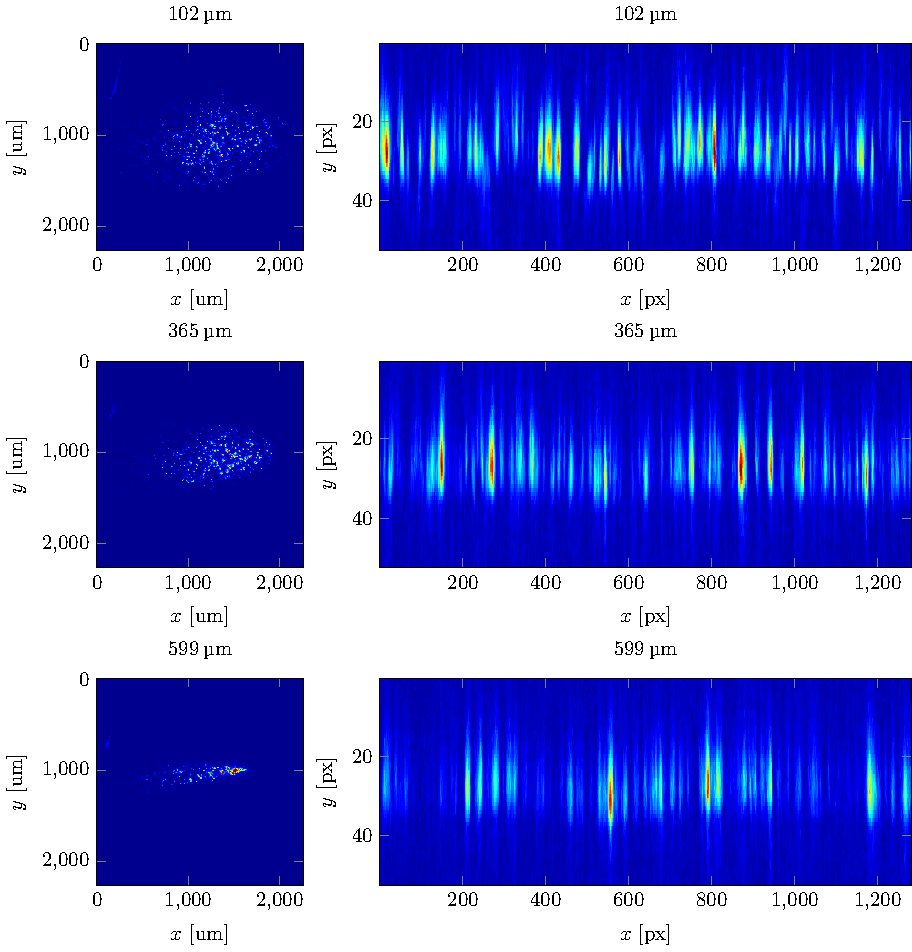
\includegraphics[keepaspectratio]{speckle/figures/spotsize/test.pdf}
\caption{Illuminated spot size (left) and corresponding specklegram (right)
for three different example spot sizes.  Notice that the angular size of the
speckles is not significantly different in the three cases.}
\label{fig:spotsizewspeckle}
\end{figure}


In \Figure{fig:spotsize} the angular size of speckles was computed for spot
sizes in the range of 100 to \SI{450}{\micro\meter} by ensemble averaging the
normalized autocovariance function across different realizations of the same
speckle pattern at the same spot size.  Surprisingly, the results show a
speckle size which is independent of spot size within this range.  The
intersection of the theoretical prediction from \Equation{eqn:angularsize} and
the experimental data occurs at a spot size of \SI{250}{\micro\meter}.  
\begin{figure}[ht]
\centering
\import{includes/}{setpgfinc}
\import{speckle/figures/spotsize/}{spotsizefig}
%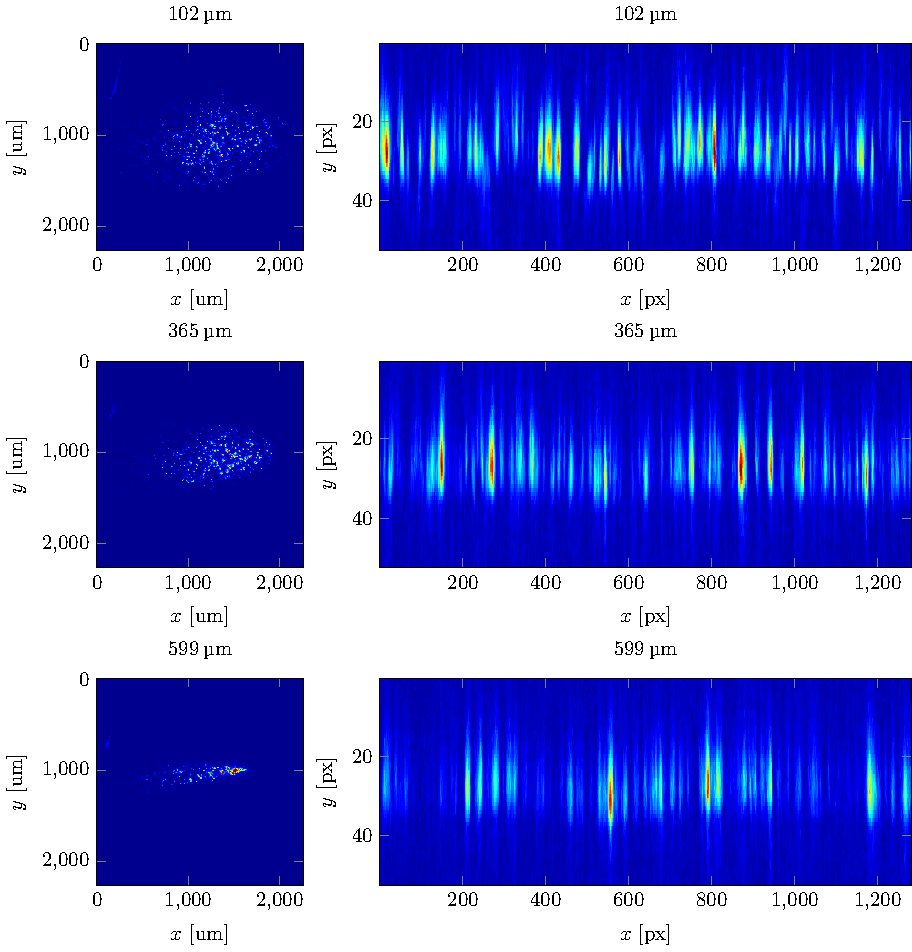
\includegraphics[keepaspectratio]{speckle/figures/spotsize/test.pdf}
\caption{Speckle size versus spot size for \SI{57}{\nano\meter} AuNPs adsorbed
onto a gold surface in a long-range surface plasmon (symmetric) structure.}
\label{fig:spotsize}
\end{figure}

This phenomena is \textit{not} present when exciting conventional surface
plasmons in a similar setup (\Figure{fig:opticalsetup}), as evidenced in
\Figure{fig:threespecklesizes} for an Air-Ag-BK7 three-layer setup (see
\Section{sec:intexperimental}).  From left to right, each image shows the cone
with a progressively tighter focal spot: on the left, a defocused spot,
center, a tightly focused spot, and right, a spot focused on a single defect
creating a ring with out speckle.  Although neither the actual spot size nor
the camera position was recorded in this particular experiment, the behavior
is clearly qualitatively described by \Equation{eqn:angularsize}; the size of
the speckle is inversely proportional to the spot size.
\begin{figure}[ht]
\centering
\begin{subfigure}[b]{5cm}
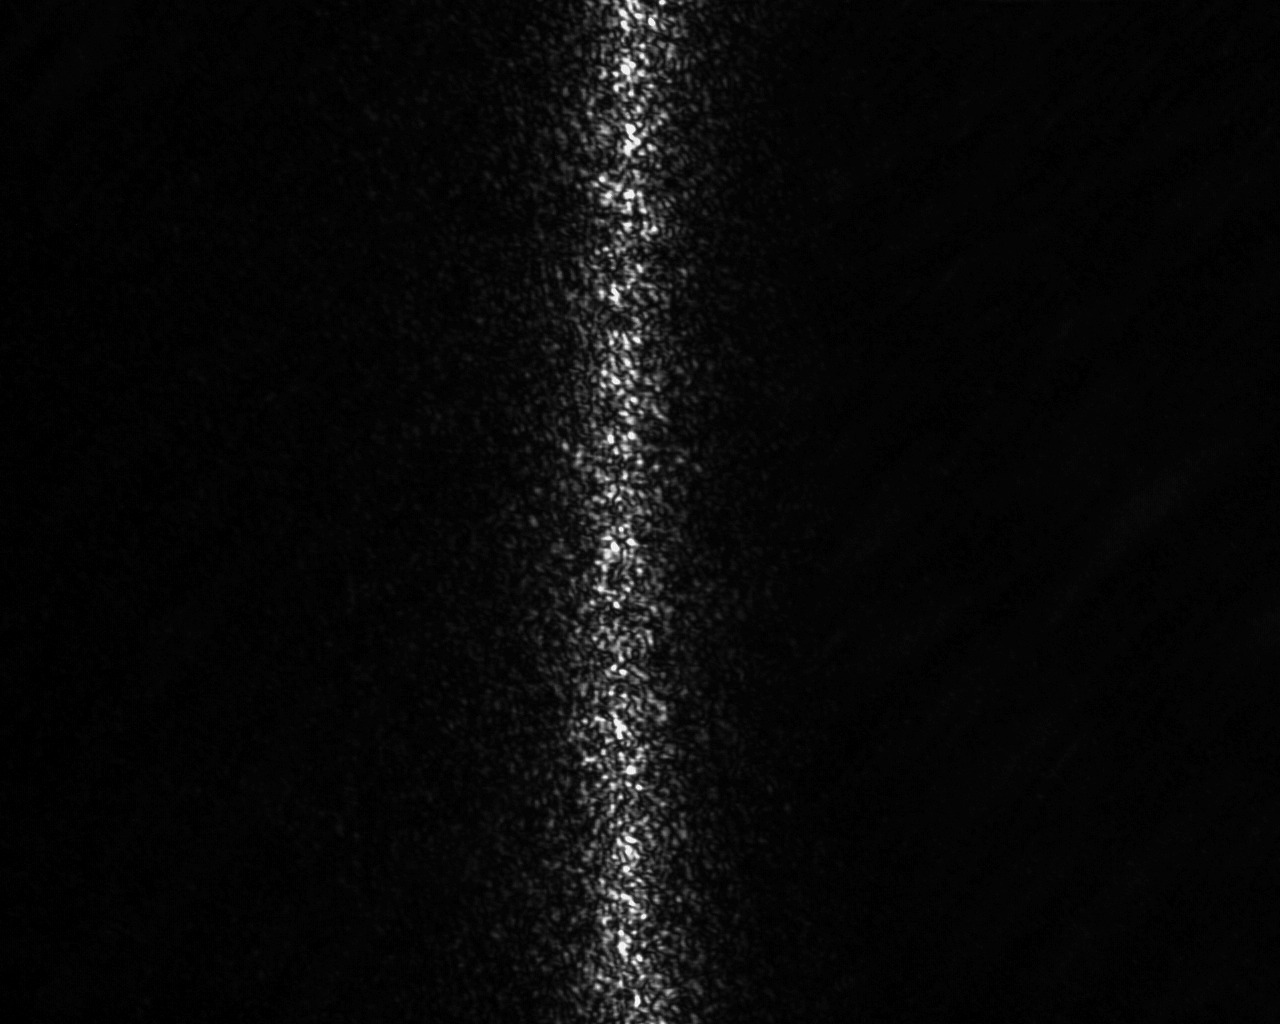
\includegraphics[keepaspectratio,width=5cm]{speckle/figures/Ag_BK7_cone_lens00_ccd-10.jpg}
\caption{defocused}
\end{subfigure}
\begin{subfigure}[b]{5cm}
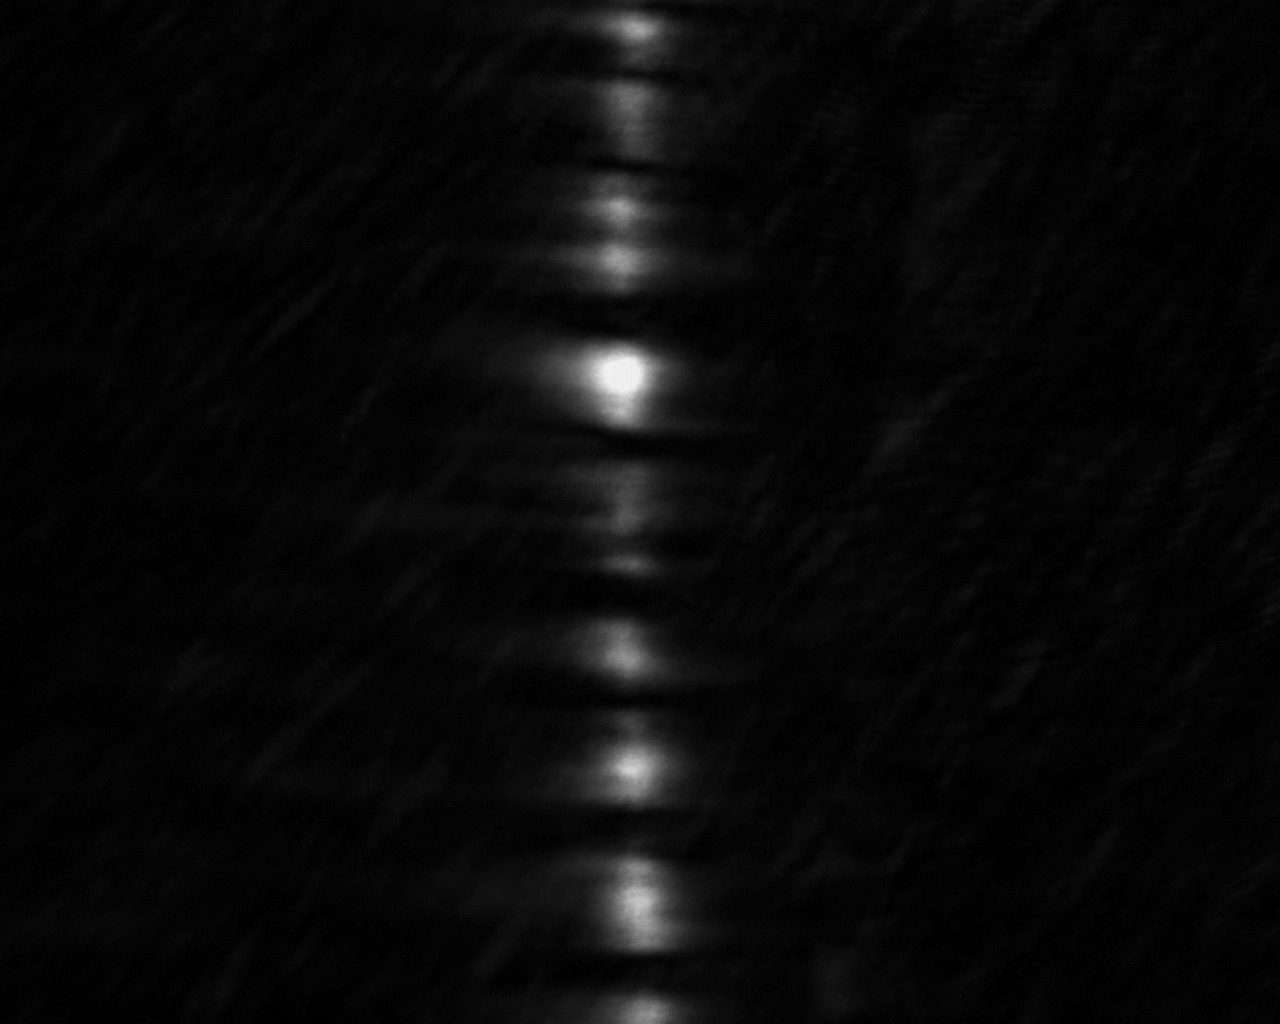
\includegraphics[keepaspectratio,width=5cm]{speckle/figures/Ag_BK7_cone_lens10_ccd-5.jpg}
\caption{tightly focused}
\end{subfigure}
\begin{subfigure}[b]{5cm}
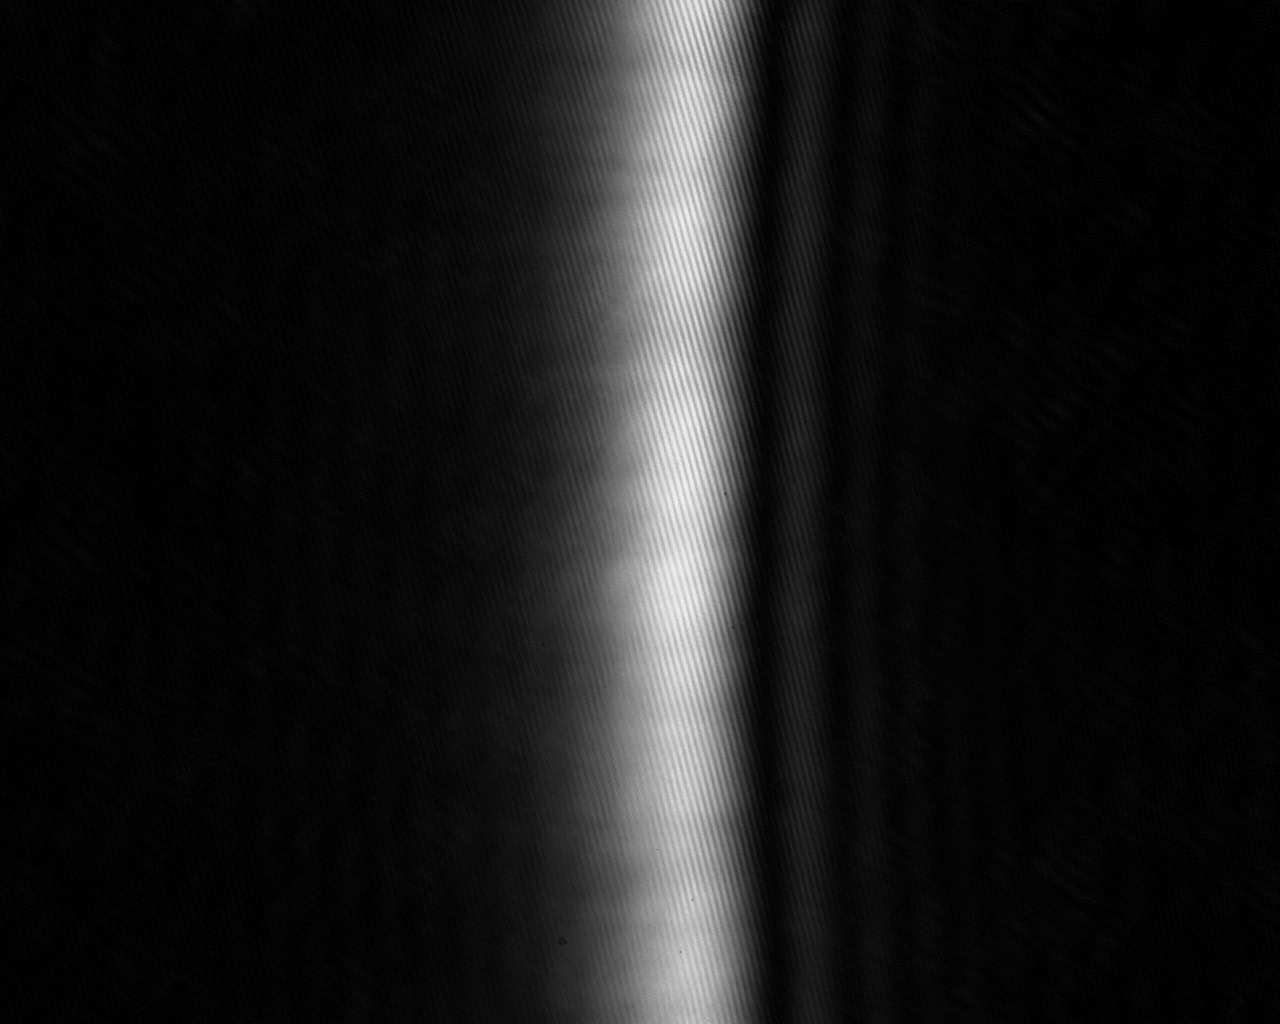
\includegraphics[keepaspectratio,width=5cm]{speckle/figures/Ag_LaSFN9_cone_lens10_ccd-153.jpg}
\caption{tightly focused on a defect}
\end{subfigure}
\caption{Three sections of cone speckle taken for a conventional surface
				plasmon setup (Air-Ag-BK7) taken using the setup of
				\Figure{fig:opticalsetup}.  The layer structure is described in
				\Section{sec:intexperimental}.  From left to right: defocused, tightly
focused, tightly focused on a defect.  The actual spot size was not measured
in this specific experiment.  }
\label{fig:threespecklesizes}
\end{figure}

\Equation{eqn:angularsize} describes an inverse relationship between speckle
size and the size of the scattering spot which is in accord with the
approximation given by \name{Dainty}~\cite{dainty1975laser} of $\lambda z/d$.  

% discrepancy stuff goes here

%MAKE SURE TO TALK ABOUT WHY NO ENHANCED SURFACE ROUGHNESS!  DO YOU HAVE ANY PICTURES?
